\documentclass[tikz]{standalone}
\begin{document}

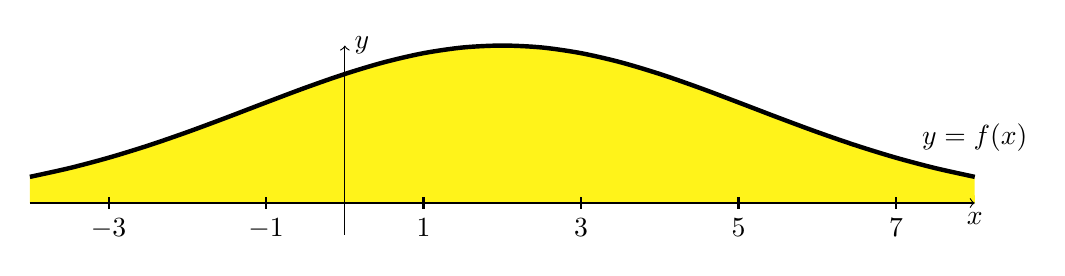
\begin{tikzpicture}[yscale=2]

  %shade region
  \fill[fill=yellow!90] plot[smooth, samples=100, domain=-4:8 ] (\x,{2.71 ^ (-(\x-2)*(\x-2)/20)})-- (8, 0) --(-4, 0)-- cycle;
    
  %draw curve
  \draw[domain=-4:8,smooth,variable=\x,black,ultra thick] plot ({\x},{2.71 ^ (-(\x-2)*(\x-2)/20)}) 
        node[above,outer sep=6pt]{$y=f(x)$};
    
  % tick marks
  \foreach \x in {-3,-1,...,7} 
    \draw [thick] (\x cm,1pt) -- (\x cm,-1pt) node[below] {$\x$};
  \foreach \y in {} 
    \draw [thick] (1pt,\y cm) -- (-1pt,\y cm) node[left] {$\y$};

  %draw axes
  \draw[->] (-4,0) -- (8,0) node[below] {$x$};
  \draw[->] (0,-0.2) -- (0,1) node[right] {$y$};

\end{tikzpicture}
\end{document} 
